\documentclass[12pt]{article}
\usepackage{geometry}
    \geometry{
        a4paper,
        lmargin=2cm,
        rmargin=2cm,
        tmargin=2cm,
        bmargin=2cm
    }
\usepackage{float}
\usepackage{indentfirst}
\usepackage{caption}
\usepackage{graphicx}
\usepackage{fontspec}
\usepackage{listings}
\usepackage{color}
\usepackage[T1]{fontenc}
\lstloadlanguages{C,C++,csh,Java}

\setmainfont[Mapping=tex-text]{Times New Roman}
\definecolor{red}{rgb}{0.6,0,0}
\definecolor{blue}{rgb}{0,0,0.6}
\definecolor{green}{rgb}{0,0.8,0}
\definecolor{cyan}{rgb}{0.0,0.6,0.6}
\renewcommand{\contentsname}{Sadržaj}

\title{Domaći 1 - Optimalni kućni poslovi}
\author{Ognjen Čavić E2 161/2024}
\date{Decembar 2024}
\begin{document}
\maketitle
\section{Opis Problema}
\par Kuvanje musake, pranje veša, pranje sudova i odlazak u kupovinu su kućni
poslovi koje čovek treba da obavi na optimalan način.
Da bi se musaka stavila na kuvanje, pre toga je neophodno spremiti sastojke što
podrazumeva seckanje luka (3 sekunde), ljuštenje i pranje krompira (5 sekundi)
i na kraju prženje mesa (7 sekundi).
Nakon što su sastojci spremni, musaka se kuva 45 sekundi.
Mašinama za pranje veša i sudova je potrebno 90 sekundi i 60 sekundi da obave
svoj posao, respektivno.
Poslednji zadatak je odlazak u kupovinu koji traje 15 sekundi.
\section{Logika rešenja}
\par Prvo što je potrebno uraditi jeste razgraničiti "aktivne" i "pasivne"
poslove.
Pasivan posao podrazumeva da nešto drugo radi umesto čoveka, on/ona treba
da uradi nešto kako bi rad počeo i nakon toga može da se posveti drugim obavezama.
Aktivan posao zahteva punu pažnju čoveka i ne dozvoljava da radi bilo šta drugo
za to vreme.
Stoga su pranje sudova, pranje veša i kuvanje musake pasivni poslovi, jer im se
"zadaje" (fizički u njih stavlja) objekat nad kojim vrše rad i dok se on ne
završi, čovek im ne posvećuje pažnju.
\par Preostale obaveze, tj. spremanje sastojaka musake i odlazak u kupovinu su
aktivni poslovi, što znači da čovek prvo treba da stavi sudove i veš na pranje,
zatim da spremi sastojke za musaku, stavi istu u rernu, potom da ode u kupovinu.
Kada se vrati iz prodavnice, sledi čekanje da se poslovi završe.
\section{Implementacija i rezultati}
\par Sobzirom da pasivni poslovi dozvoljavaju da se za vreme njihovog trajanja
rade druge stvari, oni su opisani kao \textbf{Task}-ovi.
Aktivne obaveze se pozivaju pomoću delegata \textbf{activeChore}, razlog za to
je malo uredniji kod.
Same funkcije koje opisuju izvršavanje obaveza su trivijalne, ispisuju poruku
kad počinju, nakon čega sledi čekanje, i ispisuje se kad su završene.
\par \textbf{Main} funkcija počinje pokretanjem štoperice (koja služi za ispis
i bolje praćenje izvršavanja) i pasivnih zadataka za pranje sudova i veša.
Zatim se ulazi u petlju koja obavlja aktivne poslove oko spremanja musake, koja
pre nego što se počne sledeći korak proverava da li se neki pasivni zadatak
završio pomoću funkcije \textbf{checkPassiveChoreCompletion}.
Ova funkcija iterira listu pasivnih poslova, svaki gotov posao briše iz liste
i ispisuje poruku da je čovek uradio nešto povodom završetka radnje.
Razlog za proveru završetka poslova je tu u slučaju da se dužine trajanja radnji
promeni.
\par Nakon što su sastojci spremni, sledi još jedna provera da li su pasivni
poslovi završeni i onda se musaka stavlja u rernu i čovek odlazi u kupovinu.
Kada je i to gotovo, sledi čekanje da se preostali poslovi završe, kako se koji
završi on se briše iz liste i ispisuju se odgovarajuće poruke.
\newpage
\par Na slici 1 je prikazan rezultat izvršavanja programa i vidi se da vremena
kada koji zadatak počinje i završava nisu tačna vremena kao što je zadatkom
propisano.
Razlog za to je što je kreiranje taskova i provera završetka pasivnih poslova
nije momentalno.
\begin{center}
	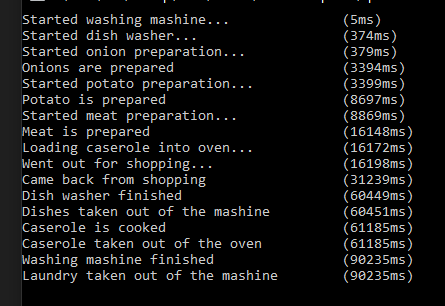
\includegraphics{figs/Rezultat.PNG}
	\captionof*{figure}{Slika 1: Rezultat izvršavanja}
\end{center}
\end{document}
